\documentclass{article}
\usepackage[utf8]{inputenc}
\usepackage{amsmath,amssymb}
\usepackage{amsfonts}
\usepackage{paralist}
\usepackage{color}
\usepackage[table]{xcolor}
\usepackage{graphicx}
\usepackage[detect-weight=true, binary-units=true]{siunitx}
\usepackage{pgfplots}
\usepackage{authblk}
\usepackage{url}
\usepackage{multirow}
\usepackage{booktabs}
\usepackage{blindtext}


\title{Introduction to Machine Learning project:\\Twitter food popularity}
\author[*]{Alessio Gaia, Carpenè Sara, Fantuzzi Giulio, Valentinis Alessio}
%\author[2]{Carpenè Sara}
%\author[3]{Fantuzzi Giulio}
%\author[4]{Valentinis Alessio}
\affil[*]{
    problem statement,
    solution design,
    solution development,
    data gathering,
    writing
}
\date{Course of AA $2023$-$2024$ - Data Science and Artificial Intelligence}



\begin{document}

\maketitle



\section{Problem statement}
\label{sec:problem_statement}
The aim of this project is to build a Machine Learning system to predict \textit{how popular} a tweet about food will be.
The dataset on which to conduct our analysis is not provided, so we are required to build one.\\
Formally, given $X$ and $Y$, defined as X = $\{x \mid x \text{ is a tweet about food}\}$ and $Y=\mathbb{R}$, our goal is to learn a model $m \in M$ from an $f'_{learn}: P^{*}(X' \times Y) \rightarrow M$ and use it into an $f'_{predict: X' \times M \rightarrow Y}$ to predict the output variable $y$.\\[0.2cm]
% Remember that we define
% \begin{align*}
% \begin{gathered}
% 	f'_{learn}: P^{*}(X' \times Y) \rightarrow M\\
% 	f'_{predict} : X' \times M \rightarrow Y.
% \end{gathered}
% \end{align*}
\textbf{Important note:} $x \in X$, being a tweet, is not directly processable by a machine. Hence, a pre-processing phase $f_{preproc}: X \rightarrow X'$ is required (add link).\\[0.2cm]
A solution based on a Machine Learning approach is suitable for this assignment: building an $f'_{learn}$ cannot be done by humans, given the nature of the problem (concerning above all complexity of the solution and human cost in dealing with thousands of observation, each with many covariates).
Furthermore, due to what described above, the model $m \in M$ will not be simple, so performing the prediction in a computer is the only suitable choice.\\
Given the nature of the problem we are opting for a regression approach and, given also the nature of $X$ and $Y$, we opted for supervised learning techniques.

% \textit{Less important note:Due to different programming backgrounds, the project has been implemented using both $R$, for preprocessing and text alaysis, and $Python$, for data gathering and model assessment.}



\section{Data}
\label{sec:data}

\subsection{Web scraping}
We are not going into details of the data-gathering process; to maximaly summarize, we used the Python library \textit{ntscraper} (insert link to reference to documentation), as it allowed us to break through X's new limitation on 1500 downloadable Tweets per month, which could have resulted in too few data. Despite this, due to the computational time of the library, especially when gathering user's information, we collected a total of $4075$ tweets containing the word '\textit{food}' and written in English.
\subsection{Preprocessing}
Each observation contains some information about the tweet: text, quotes, is.retweet, external.link, pictures, videos, gifs, multimedial.content and some information about the user: user.image, user.bio, user.website, user.tweets, user.following, user.media.
Among this variables the numerical ones are: quotes, user.tweets, user.following, user.media and the boolean ones are: is.retweet, external.link, pictures, videos, gifs, multimedial.content, user.image, user.bio, user.website.
\noindent We implemeted some customed functions to get the number of hashtags and emojis of each text, and we added them as features.\\
We performed pre-precessing on the text of tweets (conversion to lowercase, removal of punctuation, stemming, removal of stop words). Then we applied tf-idf vectorization of the preprocessed text, since it weight the importance of a word relative to the frequence across all the corpus. (penalizing common words and enhancing less common and more informative words.)
More precisely, we kept only the words in at least 40 tweets (1\% of total tweets).



\noindent Regarding the response variable, we opted for the engagement rate, i.e. a measure that keeps count of interaction (likes, comments, retweets) a post receive, over the total number of follower of the account that have published the tweet. In addition we applied a logarithmic transformation, to mitigate the resulting excessive skewness of this variable.
Formally, we used as output variable the quantity $$y^{(i)} = \ln \left( \frac{1+retweets^{(i)}+likes^{(i)}+comments^{(i)}}{1+followers^{(i)}} \right)$$
The quantity $1$ added both at numerator and denominator is applied in order not to obtain $-\infty$ or $\infty$ as values.

\section{Assessment and performance indexes}
\label{sec:assessment_performance_index}
Recalling that we are dealing with a numerical and continuous output variable $Y$, it's natural to come up with measure like Root Mean Squared Error (RMSE) to assess the techniques \textit{effectiveness}.
To deal with \textit{efficiency}, instead, we opted to evaluate the execution time of both learning and prediction phase. Times will be measured on the prediction and learning phase of the 10-fold Cross Validation used for assessing the effectiveness of the models.


\section{Proposed solution}
\label{sec:solution}

After having retrieved the data, we tested five different learning techniques, namely: (i) Dummy regressor, (ii) Regression tree, (iii) Random Forest, (iv) Support Vector Machines, (v) k-Nearest Neighbor.

\subsection{Hyper-parameter tuning}
For all of these techniques we applied hyper-parameter tuning, focusing on maximizing the \textit{effectiveness}, so minimizing a measure of error.

\noindent
\begin{minipage}{0.5\textwidth}
    \textbf{Regression Tree:} \\
    The parameter tuned is $n_{\text{min}}$, the values considered are: 1, 10, 15, 25, 30, 50, 100, 150, 200, 500. The one that minimizes the RMSE is 100.
\end{minipage}%
\begin{minipage}{0.5\textwidth}
    \centering
    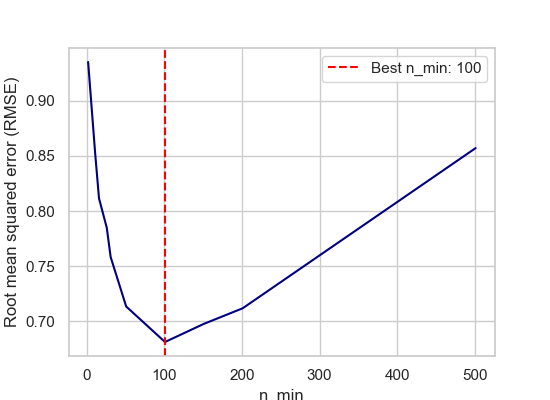
\includegraphics[scale=0.35]{dt_grid_search.png}
\end{minipage}

\noindent
\begin{minipage}{0.5\textwidth}
\textbf{Random Forest:} The parameters tuned are $n_{\text{vars}}$ and $n_{\text{min}}$. The values considered are respectively: 10, 15, 25, 50, 75, 100, 250, 500 and 1, 10, 25, 50, 75, 100. The combination that minimizes the RMSE is $n_{\text{vars}} = 500$, $n_{\text{min}} = 2$.
\end{minipage}%
\begin{minipage}{0.5\textwidth}
    \centering
    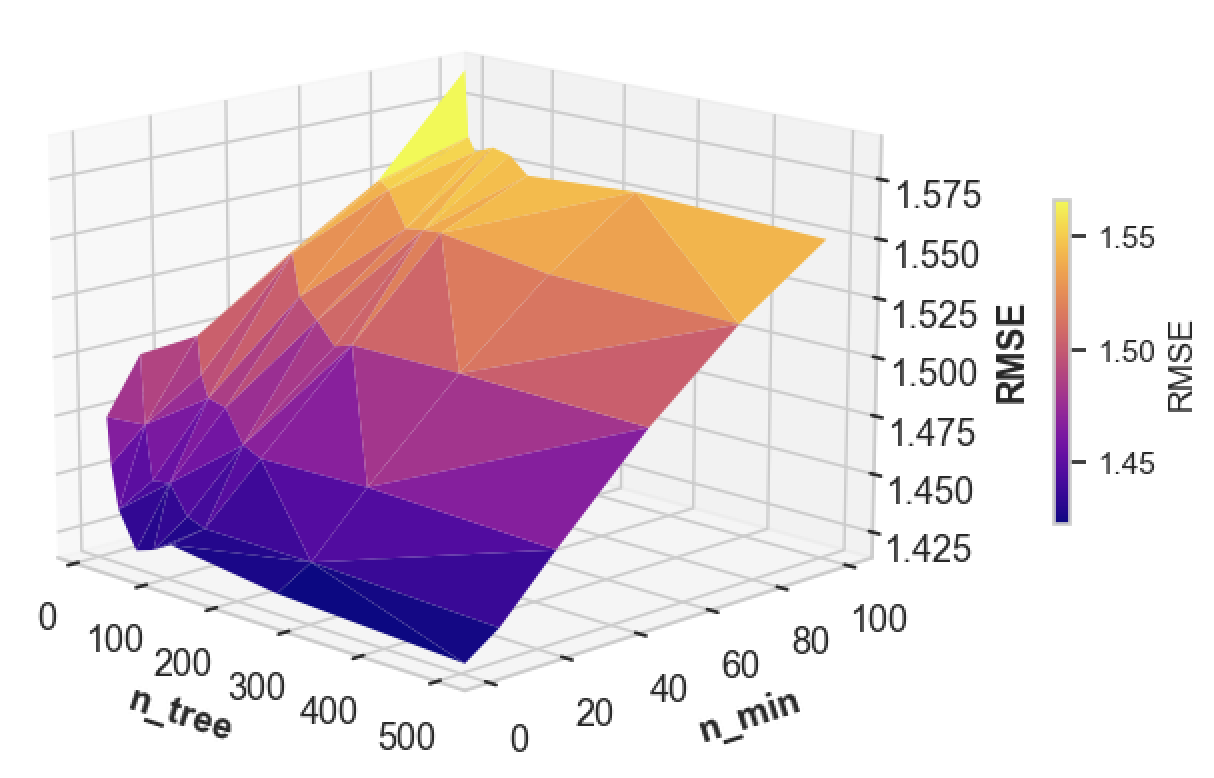
\includegraphics[scale=0.35]{rmse_vs_n_estimators_and_min_samples_split_SURFACE.png}
\end{minipage}

\noindent 


%\textbf{SVM}

\noindent
\begin{minipage}{0.5\textwidth} %
\textbf{k-Nearest Neighbor:} \\ The parameter tuned is $n_{neighbors}$, the values considered are: 1, 2, 5, 10, 15, 20, 50, 100. The one that mimimize the RMSE is 20.
The one that mimimize the RMSE is 100.
\end{minipage} %
\begin{minipage}{0.5\textwidth} %
    \centering
    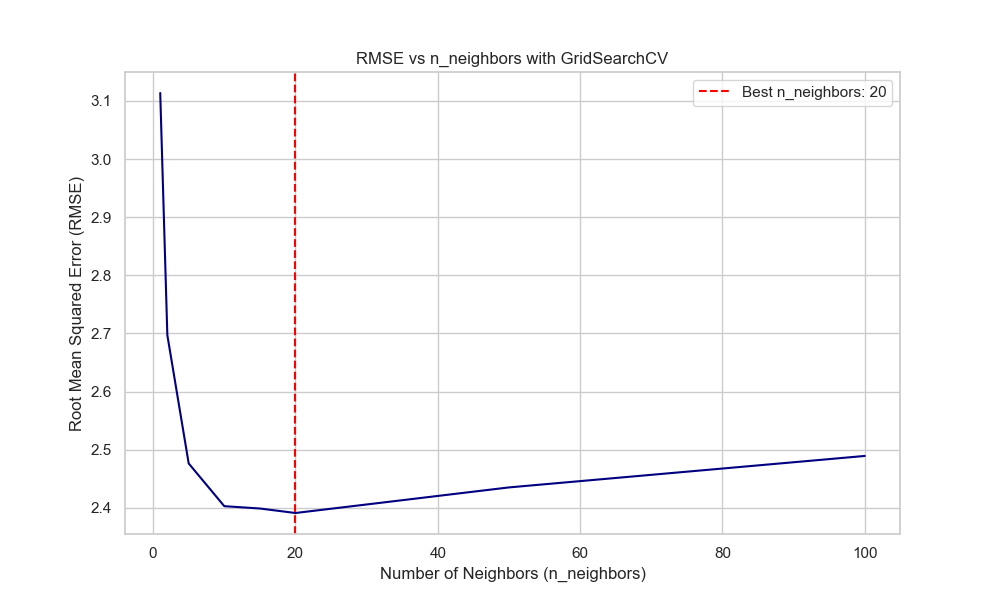
\includegraphics[scale=0.35]{knn_grid_search.png}
\end{minipage}

INSERIRE SVR!!!!!!!!!!!!!!!!!!!!!!!!!



\noindent We performed 10 fold cross validation to compare different learning techniques, in order to assess in a robus way both their effectiveness and efficiency.
\section{Results and discussion}


\begin{tabular}{c|cc|cccc|}
&\multicolumn{2}{>{\columncolor{blue!50}}c|}{\textbf{Effectiveness (RMSE)}} & \multicolumn{4}{>{\columncolor{blue!50}}c|}{\textbf{Efficiency (Time in seconds)}}\\
\multicolumn{1}{>{\columncolor{blue!50}}c|} {\textbf{Models}} & \multicolumn{1}{>{\columncolor{blue!30}}c} {$\mu$} & \multicolumn{1}{>{\columncolor{blue!30}}c|}{$\sigma$}& \multicolumn{1}{>{\columncolor{blue!30}}c}{$learn_{\mu}$}& \multicolumn{1}{>{\columncolor{blue!30}}c}{$learn_{\sigma}$}& \multicolumn{1}{>{\columncolor{blue!30}}c}{$pred_{\mu}$}& \multicolumn{1}{>{\columncolor{blue!30}}c|}{$pred_{\sigma}$} \\ 
\rowcolor{gray!10} Dummy &2.549340&0.072147&0.002053&0.000721&0.000400&0.000117 \\ 

\rowcolor{white} Reg. Tree&1.643083&0.078081&0.026919&0.002594&0.001256&0.000230\\ 

\rowcolor{gray!10} RF &1.376405&0.082878&1.072064&0.017428&0.028506&0.000607\\ 

\rowcolor{white} SVR & 2.227806&0.133183&1.582947&0.017643&0.274769&0.003610\\ 
\rowcolor{gray!10} kNN &2.359671&0.037312&0.006088&0.001386&0.032701&0.030015\\
\end{tabular}\\[0.5cm]


The table above reveals that by using the optimized parameters the best technique to tackle the problem (according to RMSE) is Random Forest. 

Obviously the most efficient method result to be the Dummy classifier, as we could imagine, but it is the most ineffective by far.
On the contrary, it's interesting to notice how on our analysis SVM performs the worst both in terms of learning and prediction, and it results in one of the worst techniques.
CITARE WISDOM OF TREES

An interesting feature might be to analyze how we can relax the parameters of RF (and trees), to see how this would effect the trade-off between efficiency and effectiveness.
INSERIRE ANALISI CON PARAMETRI NON OTTIMALI E VEDERE TEMPI ED ERRORE.
(Anotherone bites the dust)(TADA DUM    DUM    DUM)

One of the first aspects in which this analysis would get better is of course try and gather more data, which would result in a better and more precise learning phase. In fact, such a small data set would not be fully representative of the system.
If a larger data set would have been gathered, it would be interesting to perform again some hyper parameter tuning and see if the hierarchy of the techniques hols, or if some of them might gain in effectiveness (especially SVR, we trusted them :( ).

(PENSARE SE INSERIRE CONSIDERAZIONI SUL FATTO CHE STIAMO LAVORANDO SU LINGUAGGIO NATURALE E A SPANNE è UNA MERDA).
(It is also interesting to inspect how the effectiveness-efficiency trade off changes by relaxing some hyperparameters... )
\cite{slides}

\newpage
\bibliographystyle{plain}
\bibliography{bibliography}


\end{document}
